\documentclass[1p]{elsarticle_modified}
%\bibliographystyle{elsarticle-num}

%\usepackage[colorlinks]{hyperref}
%\usepackage{abbrmath_seonhwa} %\Abb, \Ascr, \Acal ,\Abf, \Afrak
\usepackage{amsfonts}
\usepackage{amssymb}
\usepackage{amsmath}
\usepackage{amsthm}
\usepackage{scalefnt}
\usepackage{amsbsy}
\usepackage{kotex}
\usepackage{caption}
\usepackage{subfig}
\usepackage{color}
\usepackage{graphicx}
\usepackage{xcolor} %% white, black, red, green, blue, cyan, magenta, yellow
\usepackage{float}
\usepackage{setspace}
\usepackage{hyperref}

\usepackage{tikz}
\usetikzlibrary{arrows}

\usepackage{multirow}
\usepackage{array} % fixed length table
\usepackage{hhline}

%%%%%%%%%%%%%%%%%%%%%
\makeatletter
\renewcommand*\env@matrix[1][\arraystretch]{%
	\edef\arraystretch{#1}%
	\hskip -\arraycolsep
	\let\@ifnextchar\new@ifnextchar
	\array{*\c@MaxMatrixCols c}}
\makeatother %https://tex.stackexchange.com/questions/14071/how-can-i-increase-the-line-spacing-in-a-matrix
%%%%%%%%%%%%%%%

\usepackage[normalem]{ulem}

\newcommand{\msout}[1]{\ifmmode\text{\sout{\ensuremath{#1}}}\else\sout{#1}\fi}
%SOURCE: \msout is \stkout macro in https://tex.stackexchange.com/questions/20609/strikeout-in-math-mode

\newcommand{\cancel}[1]{
	\ifmmode
	{\color{red}\msout{#1}}
	\else
	{\color{red}\sout{#1}}
	\fi
}

\newcommand{\add}[1]{
	{\color{blue}\uwave{#1}}
}

\newcommand{\replace}[2]{
	\ifmmode
	{\color{red}\msout{#1}}{\color{blue}\uwave{#2}}
	\else
	{\color{red}\sout{#1}}{\color{blue}\uwave{#2}}
	\fi
}

\newcommand{\Sol}{\mathcal{S}} %segment
\newcommand{\D}{D} %diagram
\newcommand{\A}{\mathcal{A}} %arc


%%%%%%%%%%%%%%%%%%%%%%%%%%%%%5 test

\def\sl{\operatorname{\textup{SL}}(2,\Cbb)}
\def\psl{\operatorname{\textup{PSL}}(2,\Cbb)}
\def\quan{\mkern 1mu \triangleright \mkern 1mu}

\theoremstyle{definition}
\newtheorem{thm}{Theorem}[section]
\newtheorem{prop}[thm]{Proposition}
\newtheorem{lem}[thm]{Lemma}
\newtheorem{ques}[thm]{Question}
\newtheorem{cor}[thm]{Corollary}
\newtheorem{defn}[thm]{Definition}
\newtheorem{exam}[thm]{Example}
\newtheorem{rmk}[thm]{Remark}
\newtheorem{alg}[thm]{Algorithm}

\newcommand{\I}{\sqrt{-1}}
\begin{document}

%\begin{frontmatter}
%
%\title{Boundary parabolic representations of knots up to 8 crossings}
%
%%% Group authors per affiliation:
%\author{Yunhi Cho} 
%\address{Department of Mathematics, University of Seoul, Seoul, Korea}
%\ead{yhcho@uos.ac.kr}
%
%
%\author{Seonhwa Kim} %\fnref{s_kim}}
%\address{Center for Geometry and Physics, Institute for Basic Science, Pohang, 37673, Korea}
%\ead{ryeona17@ibs.re.kr}
%
%\author{Hyuk Kim}
%\address{Department of Mathematical Sciences, Seoul National University, Seoul 08826, Korea}
%\ead{hyukkim@snu.ac.kr}
%
%\author{Seokbeom Yoon}
%\address{Department of Mathematical Sciences, Seoul National University, Seoul, 08826,  Korea}
%\ead{sbyoon15@snu.ac.kr}
%
%\begin{abstract}
%We find all boundary parabolic representation of knots up to 8 crossings.
%
%\end{abstract}
%\begin{keyword}
%    \MSC[2010] 57M25 
%\end{keyword}
%
%\end{frontmatter}

%\linenumbers
%\tableofcontents
%
\newcommand\colored[1]{\textcolor{white}{\rule[-0.35ex]{0.8em}{1.4ex}}\kern-0.8em\color{red} #1}%
%\newcommand\colored[1]{\textcolor{white}{ #1}\kern-2.17ex	\textcolor{white}{ #1}\kern-1.81ex	\textcolor{white}{ #1}\kern-2.15ex\color{red}#1	}

{\Large $\underline{12n_{0261}~(K12n_{0261})}$}

\setlength{\tabcolsep}{10pt}
\renewcommand{\arraystretch}{1.6}
\vspace{1cm}\begin{tabular}{m{100pt}>{\centering\arraybackslash}m{274pt}}
\multirow{5}{120pt}{
	\centering
	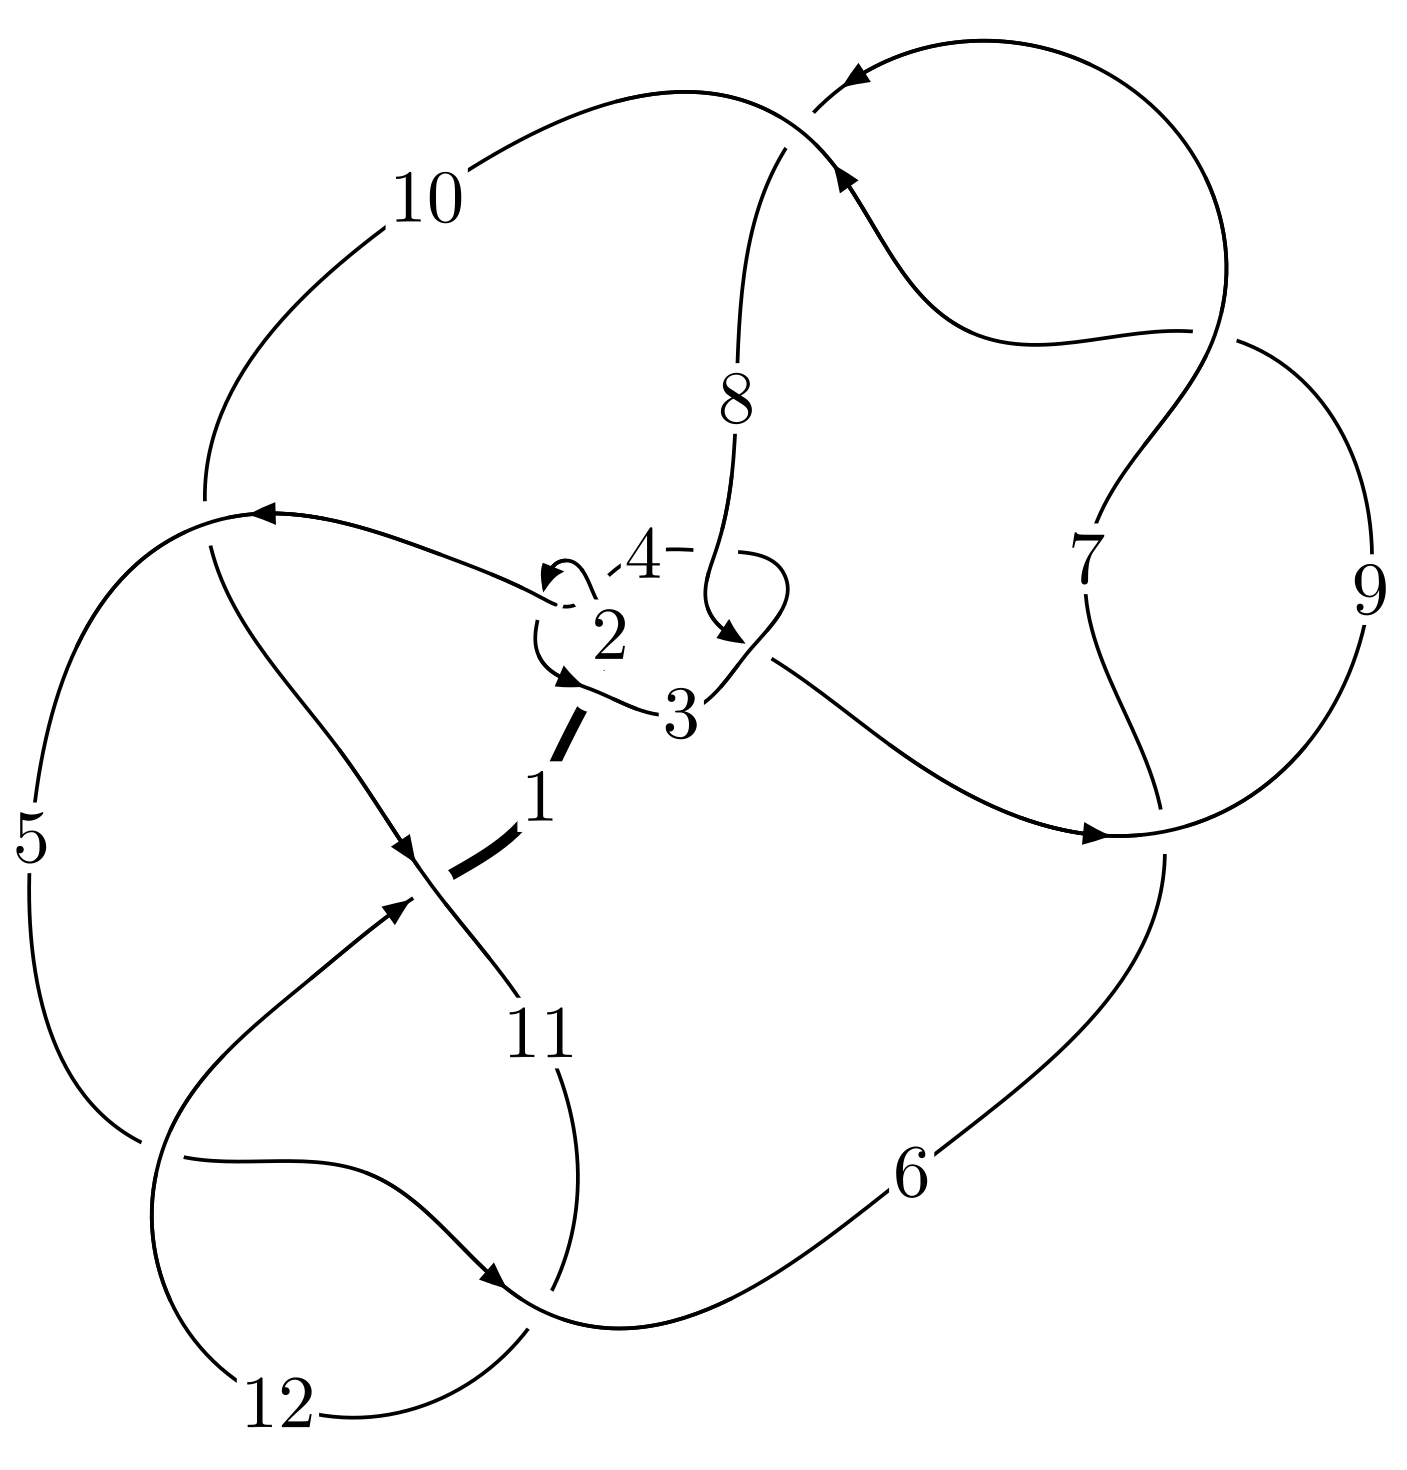
\includegraphics[width=112pt]{../../../GIT/diagram.site/Diagrams/png/2350_12n_0261.png}\\
\ \ \ A knot diagram\footnotemark}&
\allowdisplaybreaks
\textbf{Linearized knot diagam} \\
\cline{2-2}
 &
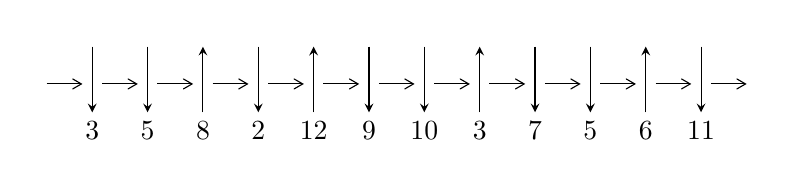
\begin{tikzpicture}[x=20pt, y=17pt]
	% nodes
	\node (C0) at (0, 0) {};
	\node (C1) at (1, 0) {};
	\node (C1U) at (1, +1) {};
	\node (C1D) at (1, -1) {3};

	\node (C2) at (2, 0) {};
	\node (C2U) at (2, +1) {};
	\node (C2D) at (2, -1) {5};

	\node (C3) at (3, 0) {};
	\node (C3U) at (3, +1) {};
	\node (C3D) at (3, -1) {8};

	\node (C4) at (4, 0) {};
	\node (C4U) at (4, +1) {};
	\node (C4D) at (4, -1) {2};

	\node (C5) at (5, 0) {};
	\node (C5U) at (5, +1) {};
	\node (C5D) at (5, -1) {12};

	\node (C6) at (6, 0) {};
	\node (C6U) at (6, +1) {};
	\node (C6D) at (6, -1) {9};

	\node (C7) at (7, 0) {};
	\node (C7U) at (7, +1) {};
	\node (C7D) at (7, -1) {10};

	\node (C8) at (8, 0) {};
	\node (C8U) at (8, +1) {};
	\node (C8D) at (8, -1) {3};

	\node (C9) at (9, 0) {};
	\node (C9U) at (9, +1) {};
	\node (C9D) at (9, -1) {7};

	\node (C10) at (10, 0) {};
	\node (C10U) at (10, +1) {};
	\node (C10D) at (10, -1) {5};

	\node (C11) at (11, 0) {};
	\node (C11U) at (11, +1) {};
	\node (C11D) at (11, -1) {6};

	\node (C12) at (12, 0) {};
	\node (C12U) at (12, +1) {};
	\node (C12D) at (12, -1) {11};
	\node (C13) at (13, 0) {};

	% arrows
	\draw[->,>={angle 60}]
	(C0) edge (C1) (C1) edge (C2) (C2) edge (C3) (C3) edge (C4) (C4) edge (C5) (C5) edge (C6) (C6) edge (C7) (C7) edge (C8) (C8) edge (C9) (C9) edge (C10) (C10) edge (C11) (C11) edge (C12) (C12) edge (C13) ;	\draw[->,>=stealth]
	(C1U) edge (C1D) (C2U) edge (C2D) (C3D) edge (C3U) (C4U) edge (C4D) (C5D) edge (C5U) (C6U) edge (C6D) (C7U) edge (C7D) (C8D) edge (C8U) (C9U) edge (C9D) (C10U) edge (C10D) (C11D) edge (C11U) (C12U) edge (C12D) ;
	\end{tikzpicture} \\
\hhline{~~} \\& 
\textbf{Solving Sequence} \\ \cline{2-2} 
 &
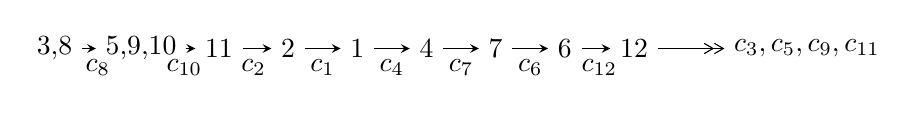
\begin{tikzpicture}[x=25pt, y=7pt]
	% node
	\node (A0) at (-1/8, 0) {3,8};
	\node (A1) at (9/8, 0) {5,9,10};
	\node (A2) at (9/4, 0) {11};
	\node (A3) at (13/4, 0) {2};
	\node (A4) at (17/4, 0) {1};
	\node (A5) at (21/4, 0) {4};
	\node (A6) at (25/4, 0) {7};
	\node (A7) at (29/4, 0) {6};
	\node (A8) at (33/4, 0) {12};
	\node (C1) at (1/2, -1) {$c_{8}$};
	\node (C2) at (7/4, -1) {$c_{10}$};
	\node (C3) at (11/4, -1) {$c_{2}$};
	\node (C4) at (15/4, -1) {$c_{1}$};
	\node (C5) at (19/4, -1) {$c_{4}$};
	\node (C6) at (23/4, -1) {$c_{7}$};
	\node (C7) at (27/4, -1) {$c_{6}$};
	\node (C8) at (31/4, -1) {$c_{12}$};
	\node (A9) at (43/4, 0) {$c_{3},c_{5},c_{9},c_{11}$};

	% edge
	\draw[->,>=stealth]	
	(A0) edge (A1) (A1) edge (A2) (A2) edge (A3) (A3) edge (A4) (A4) edge (A5) (A5) edge (A6) (A6) edge (A7) (A7) edge (A8) ;
	\draw[->>,>={angle 60}]	
	(A8) edge (A9);
\end{tikzpicture} \\ 

\end{tabular} \\

\footnotetext{
The image of knot diagram is generated by the software ``\textbf{Draw programme}" developed by Andrew Bartholomew(\url{http://www.layer8.co.uk/maths/draw/index.htm\#Running-draw}), where we modified some parts for our purpose(\url{https://github.com/CATsTAILs/LinksPainter}).
}\phantom \\ \newline 
\centering \textbf{Ideals for irreducible components\footnotemark of $X_{\text{par}}$} 
 
\begin{align*}
I^u_{1}&=\langle 
5.82214\times10^{22} u^{20}-3.29635\times10^{23} u^{19}+\cdots+1.18107\times10^{25} d-1.00440\times10^{25},\\
\phantom{I^u_{1}}&\phantom{= \langle  }-6.72232\times10^{22} u^{20}+3.09213\times10^{23} u^{19}+\cdots+2.36214\times10^{25} c-1.53724\times10^{25},\\
\phantom{I^u_{1}}&\phantom{= \langle  }5.37718\times10^{22} u^{20}-1.64184\times10^{23} u^{19}+\cdots+1.18107\times10^{25} b+1.07557\times10^{24},\\
\phantom{I^u_{1}}&\phantom{= \langle  }-6.27749\times10^{23} u^{20}+1.76680\times10^{24} u^{19}+\cdots+2.36214\times10^{25} a-1.96176\times10^{25},\\
\phantom{I^u_{1}}&\phantom{= \langle  }u^{21}-3 u^{20}+\cdots-32 u+32\rangle \\
I^u_{2}&=\langle 
-182575 u^{12}-264525 u^{11}+\cdots+1396412 d-304734,\\
\phantom{I^u_{2}}&\phantom{= \langle  }1091678 u^{12} a-2056829 u^{12}+\cdots+8227316 a+8353986,\\
\phantom{I^u_{2}}&\phantom{= \langle  }182575 u^{12} a-236482 u^{12}+\cdots-1091678 a-1127628,\\
\phantom{I^u_{2}}&\phantom{= \langle  }152367 u^{12} a-563814 u^{12}+\cdots-1320834 a+1767620,\\
\phantom{I^u_{2}}&\phantom{= \langle  }u^{13}+u^{12}+8 u^{11}+7 u^{10}+22 u^9+18 u^8+20 u^7+21 u^6- u^5+5 u^4+8 u^3-9 u^2+4 u-4\rangle \\
\\
I^v_{1}&=\langle 
a,\;d,\;c-1,\;b+v+1,\;v^2+v+1\rangle \\
I^v_{2}&=\langle 
c,\;d-1,\;b,\;a- v,\;v^2+v+1\rangle \\
I^v_{3}&=\langle 
a,\;d-1,\;c+a,\;b+1,\;v+1\rangle \\
I^v_{4}&=\langle 
c,\;d-1,\;a^2 v^2-2 c a v- v^2 a+c^2+c v+v^2,\;b v-1\rangle \\
\end{align*}
\raggedright * 5 irreducible components of $\dim_{\mathbb{C}}=0$, with total 52 representations.\\
\raggedright * 1 irreducible components of $\dim_{\mathbb{C}}=1$ \\
\footnotetext{All coefficients of polynomials are rational numbers. But the coefficients are sometimes approximated in decimal forms when there is not enough margin.}
\newpage
\renewcommand{\arraystretch}{1}
\centering \section*{I. $I^u_{1}= \langle 5.82\times10^{22} u^{20}-3.30\times10^{23} u^{19}+\cdots+1.18\times10^{25} d-1.00\times10^{25},\;-6.72\times10^{22} u^{20}+3.09\times10^{23} u^{19}+\cdots+2.36\times10^{25} c-1.54\times10^{25},\;5.38\times10^{22} u^{20}-1.64\times10^{23} u^{19}+\cdots+1.18\times10^{25} b+1.08\times10^{24},\;-6.28\times10^{23} u^{20}+1.77\times10^{24} u^{19}+\cdots+2.36\times10^{25} a-1.96\times10^{25},\;u^{21}-3 u^{20}+\cdots-32 u+32 \rangle$}
\flushleft \textbf{(i) Arc colorings}\\
\begin{tabular}{m{7pt} m{180pt} m{7pt} m{180pt} }
\flushright $a_{3}=$&$\begin{pmatrix}0\\u\end{pmatrix}$ \\
\flushright $a_{8}=$&$\begin{pmatrix}1\\0\end{pmatrix}$ \\
\flushright $a_{5}=$&$\begin{pmatrix}0.0265755 u^{20}-0.0747968 u^{19}+\cdots+1.58156 u+0.830504\\-0.00455281 u^{20}+0.0139013 u^{19}+\cdots+0.741851 u-0.0910676\end{pmatrix}$ \\
\flushright $a_{9}=$&$\begin{pmatrix}1\\- u^2\end{pmatrix}$ \\
\flushright $a_{10}=$&$\begin{pmatrix}0.00284586 u^{20}-0.0130904 u^{19}+\cdots+0.686169 u+0.650783\\-0.00492955 u^{20}+0.0279099 u^{19}+\cdots-1.68092 u+0.850415\end{pmatrix}$ \\
\flushright $a_{11}=$&$\begin{pmatrix}-0.0210595 u^{20}+0.0850046 u^{19}+\cdots-3.46686 u+1.92380\\-0.00576337 u^{20}+0.0431394 u^{19}+\cdots-2.97976 u+1.42272\end{pmatrix}$ \\
\flushright $a_{2}=$&$\begin{pmatrix}-0.0311283 u^{20}+0.0886981 u^{19}+\cdots-0.839713 u-0.921571\\-0.00455281 u^{20}+0.0139013 u^{19}+\cdots+0.741851 u-0.0910676\end{pmatrix}$ \\
\flushright $a_{1}=$&$\begin{pmatrix}-0.0311283 u^{20}+0.0886981 u^{19}+\cdots-0.839713 u-0.921571\\-0.0204279 u^{20}+0.0622591 u^{19}+\cdots-0.104280 u-0.241041\end{pmatrix}$ \\
\flushright $a_{4}=$&$\begin{pmatrix}u\\u\end{pmatrix}$ \\
\flushright $a_{7}=$&$\begin{pmatrix}0.00284586 u^{20}-0.0130904 u^{19}+\cdots+0.686169 u+0.650783\\0.00468667 u^{20}-0.0299351 u^{19}+\cdots+1.91768 u-0.996105\end{pmatrix}$ \\
\flushright $a_{6}=$&$\begin{pmatrix}0.00777542 u^{20}-0.0410003 u^{19}+\cdots+2.36709 u-0.199631\\0.00392727 u^{20}-0.0344353 u^{19}+\cdots+2.49530 u-1.41598\end{pmatrix}$ \\
\flushright $a_{12}=$&$\begin{pmatrix}-0.00320223 u^{20}+0.0332571 u^{19}+\cdots-2.57523 u+0.998926\\0.0165563 u^{20}-0.0374854 u^{19}+\cdots+0.0371713 u+0.859283\end{pmatrix}$\\&\end{tabular}
\flushleft \textbf{(ii) Obstruction class $= -1$}\\~\\
\flushleft \textbf{(iii) Cusp Shapes $= -\frac{203971647344418191706557}{1476335887006576019057698} u^{20}+\frac{2056765698754565732069615}{5905343548026304076230792} u^{19}+\cdots+\frac{11041294381070090419087484}{738167943503288009528849} u-\frac{9937042912284907740395116}{738167943503288009528849}$}\\~\\
\newpage\renewcommand{\arraystretch}{1}
\flushleft \textbf{(iv) u-Polynomials at the component}\newline \\
\begin{tabular}{m{50pt}|m{274pt}}
Crossings & \hspace{64pt}u-Polynomials at each crossing \\
\hline $$\begin{aligned}c_{1}\end{aligned}$$&$\begin{aligned}
&u^{21}+31 u^{20}+\cdots-4 u+1
\end{aligned}$\\
\hline $$\begin{aligned}c_{2},c_{4},c_{6}\\c_{7},c_{9}\end{aligned}$$&$\begin{aligned}
&u^{21}-5 u^{20}+\cdots-2 u+1
\end{aligned}$\\
\hline $$\begin{aligned}c_{3},c_{8}\end{aligned}$$&$\begin{aligned}
&u^{21}+3 u^{20}+\cdots-32 u-32
\end{aligned}$\\
\hline $$\begin{aligned}c_{5},c_{11}\end{aligned}$$&$\begin{aligned}
&u^{21}+u^{20}+\cdots-12 u-4
\end{aligned}$\\
\hline $$\begin{aligned}c_{10}\end{aligned}$$&$\begin{aligned}
&u^{21}- u^{20}+\cdots-636 u-612
\end{aligned}$\\
\hline $$\begin{aligned}c_{12}\end{aligned}$$&$\begin{aligned}
&u^{21}+11 u^{20}+\cdots+40 u-16
\end{aligned}$\\
\hline
\end{tabular}\\~\\
\newpage\renewcommand{\arraystretch}{1}
\flushleft \textbf{(v) Riley Polynomials at the component}\newline \\
\begin{tabular}{m{50pt}|m{274pt}}
Crossings & \hspace{64pt}Riley Polynomials at each crossing \\
\hline $$\begin{aligned}c_{1}\end{aligned}$$&$\begin{aligned}
&y^{21}-71 y^{20}+\cdots-144 y-1
\end{aligned}$\\
\hline $$\begin{aligned}c_{2},c_{4},c_{6}\\c_{7},c_{9}\end{aligned}$$&$\begin{aligned}
&y^{21}-31 y^{20}+\cdots-4 y-1
\end{aligned}$\\
\hline $$\begin{aligned}c_{3},c_{8}\end{aligned}$$&$\begin{aligned}
&y^{21}+15 y^{20}+\cdots-4096 y-1024
\end{aligned}$\\
\hline $$\begin{aligned}c_{5},c_{11}\end{aligned}$$&$\begin{aligned}
&y^{21}+11 y^{20}+\cdots+40 y-16
\end{aligned}$\\
\hline $$\begin{aligned}c_{10}\end{aligned}$$&$\begin{aligned}
&y^{21}-13 y^{20}+\cdots+1093608 y-374544
\end{aligned}$\\
\hline $$\begin{aligned}c_{12}\end{aligned}$$&$\begin{aligned}
&y^{21}- y^{20}+\cdots+3616 y-256
\end{aligned}$\\
\hline
\end{tabular}\\~\\
\newpage\flushleft \textbf{(vi) Complex Volumes and Cusp Shapes}
$$\begin{array}{c|c|c}  
\text{Solutions to }I^u_{1}& \I (\text{vol} + \sqrt{-1}CS) & \text{Cusp shape}\\
 \hline 
\begin{aligned}
u &= \phantom{-}0.036987 + 1.146540 I \\
a &= \phantom{-}0.578318 + 0.602865 I \\
b &= -0.222232 + 0.595413 I \\
c &= \phantom{-}0.512526 + 0.210362 I \\
d &= \phantom{-}0.669819 - 0.685364 I\end{aligned}
 & -3.32924 + 4.98790 I & -8.89610 - 7.00933 I \\ \hline\begin{aligned}
u &= \phantom{-}0.036987 - 1.146540 I \\
a &= \phantom{-}0.578318 - 0.602865 I \\
b &= -0.222232 - 0.595413 I \\
c &= \phantom{-}0.512526 - 0.210362 I \\
d &= \phantom{-}0.669819 + 0.685364 I\end{aligned}
 & -3.32924 - 4.98790 I & -8.89610 + 7.00933 I \\ \hline\begin{aligned}
u &= -0.154679 + 0.793727 I \\
a &= -0.412466 + 0.647829 I \\
b &= \phantom{-}0.050314 + 0.532414 I \\
c &= \phantom{-}0.634334 - 0.187007 I \\
d &= \phantom{-}0.450400 + 0.427591 I\end{aligned}
 & -0.57334 - 1.34767 I & -3.83291 + 5.35474 I \\ \hline\begin{aligned}
u &= -0.154679 - 0.793727 I \\
a &= -0.412466 - 0.647829 I \\
b &= \phantom{-}0.050314 - 0.532414 I \\
c &= \phantom{-}0.634334 + 0.187007 I \\
d &= \phantom{-}0.450400 - 0.427591 I\end{aligned}
 & -0.57334 + 1.34767 I & -3.83291 - 5.35474 I \\ \hline\begin{aligned}
u &= -0.470495 + 0.448103 I \\
a &= -0.409901 + 0.397885 I \\
b &= -0.268303 + 0.555704 I \\
c &= \phantom{-}0.888871 - 0.334537 I \\
d &= -0.014563 + 0.370881 I\end{aligned}
 & \phantom{-}0.53740 - 1.37698 I & \phantom{-}1.82779 + 4.46485 I \\ \hline\begin{aligned}
u &= -0.470495 - 0.448103 I \\
a &= -0.409901 - 0.397885 I \\
b &= -0.268303 - 0.555704 I \\
c &= \phantom{-}0.888871 + 0.334537 I \\
d &= -0.014563 - 0.370881 I\end{aligned}
 & \phantom{-}0.53740 + 1.37698 I & \phantom{-}1.82779 - 4.46485 I\\
 \hline 
 \end{array}$$\newpage$$\begin{array}{c|c|c}  
\text{Solutions to }I^u_{1}& \I (\text{vol} + \sqrt{-1}CS) & \text{Cusp shape}\\
 \hline 
\begin{aligned}
u &= -0.128491 + 0.614288 I \\
a &= \phantom{-}0.535926 + 1.193030 I \\
b &= -0.103617 + 0.330827 I \\
c &= \phantom{-}0.549782 + 0.053680 I \\
d &= \phantom{-}0.801726 - 0.175920 I\end{aligned}
 & -2.84340 - 1.62330 I & -11.63179 + 1.59969 I \\ \hline\begin{aligned}
u &= -0.128491 - 0.614288 I \\
a &= \phantom{-}0.535926 - 1.193030 I \\
b &= -0.103617 - 0.330827 I \\
c &= \phantom{-}0.549782 - 0.053680 I \\
d &= \phantom{-}0.801726 + 0.175920 I\end{aligned}
 & -2.84340 + 1.62330 I & -11.63179 - 1.59969 I \\ \hline\begin{aligned}
u &= \phantom{-}0.518224 + 0.162575 I \\
a &= \phantom{-}0.507737 + 0.210413 I \\
b &= \phantom{-}0.583653 + 0.355856 I \\
c &= \phantom{-}1.221470 + 0.303490 I \\
d &= -0.228914 - 0.191587 I\end{aligned}
 & -0.25092 - 2.48183 I & \phantom{-}1.69657 + 3.99164 I \\ \hline\begin{aligned}
u &= \phantom{-}0.518224 - 0.162575 I \\
a &= \phantom{-}0.507737 - 0.210413 I \\
b &= \phantom{-}0.583653 - 0.355856 I \\
c &= \phantom{-}1.221470 - 0.303490 I \\
d &= -0.228914 + 0.191587 I\end{aligned}
 & -0.25092 + 2.48183 I & \phantom{-}1.69657 - 3.99164 I \\ \hline\begin{aligned}
u &= -1.63718\phantom{ +0.000000I} \\
a &= \phantom{-}0.993823\phantom{ +0.000000I} \\
b &= -0.623198\phantom{ +0.000000I} \\
c &= \phantom{-}0.380652\phantom{ +0.000000I} \\
d &= \phantom{-}1.62707\phantom{ +0.000000I}\end{aligned}
 & -10.0156\phantom{ +0.000000I} & -8.03320\phantom{ +0.000000I} \\ \hline\begin{aligned}
u &= -0.11848 + 1.68160 I \\
a &= -0.035721 - 0.977610 I \\
b &= -0.04009 - 2.59088 I \\
c &= -1.53144 + 0.13174 I \\
d &= -1.64818 - 0.05576 I\end{aligned}
 & -10.91870 - 3.26339 I & -9.90010 + 2.49959 I\\
 \hline 
 \end{array}$$\newpage$$\begin{array}{c|c|c}  
\text{Solutions to }I^u_{1}& \I (\text{vol} + \sqrt{-1}CS) & \text{Cusp shape}\\
 \hline 
\begin{aligned}
u &= -0.11848 - 1.68160 I \\
a &= -0.035721 + 0.977610 I \\
b &= -0.04009 + 2.59088 I \\
c &= -1.53144 - 0.13174 I \\
d &= -1.64818 + 0.05576 I\end{aligned}
 & -10.91870 + 3.26339 I & -9.90010 - 2.49959 I \\ \hline\begin{aligned}
u &= \phantom{-}1.80226 + 0.29000 I \\
a &= -0.934416 + 0.075142 I \\
b &= \phantom{-}0.669749 + 0.073622 I \\
c &= \phantom{-}0.368644 - 0.018467 I \\
d &= \phantom{-}1.70586 + 0.13555 I\end{aligned}
 & -14.0445 - 5.1370 I & -11.02836 + 2.94498 I \\ \hline\begin{aligned}
u &= \phantom{-}1.80226 - 0.29000 I \\
a &= -0.934416 - 0.075142 I \\
b &= \phantom{-}0.669749 - 0.073622 I \\
c &= \phantom{-}0.368644 + 0.018467 I \\
d &= \phantom{-}1.70586 - 0.13555 I\end{aligned}
 & -14.0445 + 5.1370 I & -11.02836 - 2.94498 I \\ \hline\begin{aligned}
u &= -0.77417 + 1.65700 I \\
a &= -0.199071 - 0.900171 I \\
b &= -0.19629 - 2.45464 I \\
c &= -1.170520 + 0.665347 I \\
d &= -1.64570 - 0.36703 I\end{aligned}
 & -15.0920 - 8.4883 I & -8.50111 + 3.29621 I \\ \hline\begin{aligned}
u &= -0.77417 - 1.65700 I \\
a &= -0.199071 + 0.900171 I \\
b &= -0.19629 + 2.45464 I \\
c &= -1.170520 - 0.665347 I \\
d &= -1.64570 + 0.36703 I\end{aligned}
 & -15.0920 + 8.4883 I & -8.50111 - 3.29621 I \\ \hline\begin{aligned}
u &= \phantom{-}0.94230 + 1.60086 I \\
a &= \phantom{-}0.234926 - 0.876218 I \\
b &= \phantom{-}0.22253 - 2.40487 I \\
c &= -1.054920 - 0.759955 I \\
d &= -1.62407 + 0.44958 I\end{aligned}
 & -18.0417 + 14.4957 I & -10.41632 - 6.77876 I\\
 \hline 
 \end{array}$$\newpage$$\begin{array}{c|c|c}  
\text{Solutions to }I^u_{1}& \I (\text{vol} + \sqrt{-1}CS) & \text{Cusp shape}\\
 \hline 
\begin{aligned}
u &= \phantom{-}0.94230 - 1.60086 I \\
a &= \phantom{-}0.234926 + 0.876218 I \\
b &= \phantom{-}0.22253 + 2.40487 I \\
c &= -1.054920 + 0.759955 I \\
d &= -1.62407 - 0.44958 I\end{aligned}
 & -18.0417 - 14.4957 I & -10.41632 + 6.77876 I \\ \hline\begin{aligned}
u &= \phantom{-}0.66513 + 1.94791 I \\
a &= \phantom{-}0.137757 - 0.866713 I \\
b &= \phantom{-}0.11588 - 2.45183 I \\
c &= -1.109070 - 0.438193 I \\
d &= -1.77991 + 0.30814 I\end{aligned}
 & \phantom{-}18.5711 + 4.0668 I & -12.30105 - 1.16982 I \\ \hline\begin{aligned}
u &= \phantom{-}0.66513 - 1.94791 I \\
a &= \phantom{-}0.137757 + 0.866713 I \\
b &= \phantom{-}0.11588 + 2.45183 I \\
c &= -1.109070 + 0.438193 I \\
d &= -1.77991 - 0.30814 I\end{aligned}
 & \phantom{-}18.5711 - 4.0668 I & -12.30105 + 1.16982 I\\
 \hline 
 \end{array}$$\newpage\newpage\renewcommand{\arraystretch}{1}
\centering \section*{II. $I^u_{2}= \langle -1.83\times10^{5} u^{12}-2.65\times10^{5} u^{11}+\cdots+1.40\times10^{6} d-3.05\times10^{5},\;1.09\times10^{6} a u^{12}-2.06\times10^{6} u^{12}+\cdots+8.23\times10^{6} a+8.35\times10^{6},\;1.83\times10^{5} a u^{12}-2.36\times10^{5} u^{12}+\cdots-1.09\times10^{6} a-1.13\times10^{6},\;1.52\times10^{5} a u^{12}-5.64\times10^{5} u^{12}+\cdots-1.32\times10^{6} a+1.77\times10^{6},\;u^{13}+u^{12}+\cdots+4 u-4 \rangle$}
\flushleft \textbf{(i) Arc colorings}\\
\begin{tabular}{m{7pt} m{180pt} m{7pt} m{180pt} }
\flushright $a_{3}=$&$\begin{pmatrix}0\\u\end{pmatrix}$ \\
\flushright $a_{8}=$&$\begin{pmatrix}1\\0\end{pmatrix}$ \\
\flushright $a_{5}=$&$\begin{pmatrix}a\\-0.130746 a u^{12}+0.169350 u^{12}+\cdots+0.781774 a+0.807518\end{pmatrix}$ \\
\flushright $a_{9}=$&$\begin{pmatrix}1\\- u^2\end{pmatrix}$ \\
\flushright $a_{10}=$&$\begin{pmatrix}-0.195443 a u^{12}+0.368235 u^{12}+\cdots-1.47294 a-1.49562\\0.130746 u^{12}+0.189432 u^{11}+\cdots-0.691165 u+0.218226\end{pmatrix}$ \\
\flushright $a_{11}=$&$\begin{pmatrix}-0.169350 a u^{12}+0.368235 u^{12}+\cdots-0.807518 a-1.49562\\0.0521873 a u^{12}+0.261492 u^{12}+\cdots+1.33084 a-0.563547\end{pmatrix}$ \\
\flushright $a_{2}=$&$\begin{pmatrix}-0.130746 a u^{12}+0.169350 u^{12}+\cdots-0.218226 a+0.807518\\-0.130746 a u^{12}+0.169350 u^{12}+\cdots+0.781774 a+0.807518\end{pmatrix}$ \\
\flushright $a_{1}=$&$\begin{pmatrix}-0.130746 a u^{12}+0.169350 u^{12}+\cdots-0.218226 a+0.807518\\-0.112072 a u^{12}+0.214783 u^{12}+\cdots+1.01652 a+1.16237\end{pmatrix}$ \\
\flushright $a_{4}=$&$\begin{pmatrix}u\\u\end{pmatrix}$ \\
\flushright $a_{7}=$&$\begin{pmatrix}-0.195443 a u^{12}+0.368235 u^{12}+\cdots-1.47294 a-1.49562\\-0.0586861 a u^{12}-0.0773597 a u^{11}+\cdots-0.522983 a-1\end{pmatrix}$ \\
\flushright $a_{6}=$&$\begin{pmatrix}-0.195443 a u^{12}+0.237489 u^{12}+\cdots-1.47294 a-1.71384\\-0.0586861 a u^{12}+0.0186736 u^{12}+\cdots-0.522983 a-0.765256\end{pmatrix}$ \\
\flushright $a_{12}=$&$\begin{pmatrix}-0.280165 a u^{12}+0.0140927 u^{12}+\cdots+0.328803 a-1.76474\\-0.00702658 a u^{12}+0.208441 u^{12}+\cdots+1.44074 a-0.142777\end{pmatrix}$\\&\end{tabular}
\flushleft \textbf{(ii) Obstruction class $= -1$}\\~\\
\flushleft \textbf{(iii) Cusp Shapes $= \frac{498055}{698206} u^{12}+\frac{527627}{698206} u^{11}+\cdots-\frac{3711195}{698206} u-\frac{2197714}{349103}$}\\~\\
\newpage\renewcommand{\arraystretch}{1}
\flushleft \textbf{(iv) u-Polynomials at the component}\newline \\
\begin{tabular}{m{50pt}|m{274pt}}
Crossings & \hspace{64pt}u-Polynomials at each crossing \\
\hline $$\begin{aligned}c_{1}\end{aligned}$$&$\begin{aligned}
&u^{26}+23 u^{25}+\cdots+1824 u+256
\end{aligned}$\\
\hline $$\begin{aligned}c_{2},c_{4},c_{6}\\c_{7},c_{9}\end{aligned}$$&$\begin{aligned}
&u^{26}-3 u^{25}+\cdots-24 u-16
\end{aligned}$\\
\hline $$\begin{aligned}c_{3},c_{8}\end{aligned}$$&$\begin{aligned}
&(u^{13}- u^{12}+\cdots+4 u+4)^{2}
\end{aligned}$\\
\hline $$\begin{aligned}c_{5},c_{11}\end{aligned}$$&$\begin{aligned}
&(u^{13}+2 u^{12}+\cdots+u-1)^{2}
\end{aligned}$\\
\hline $$\begin{aligned}c_{10}\end{aligned}$$&$\begin{aligned}
&(u^{13}-2 u^{12}+\cdots+3 u-1)^{2}
\end{aligned}$\\
\hline $$\begin{aligned}c_{12}\end{aligned}$$&$\begin{aligned}
&(u^{13}+8 u^{12}+\cdots+5 u-1)^{2}
\end{aligned}$\\
\hline
\end{tabular}\\~\\
\newpage\renewcommand{\arraystretch}{1}
\flushleft \textbf{(v) Riley Polynomials at the component}\newline \\
\begin{tabular}{m{50pt}|m{274pt}}
Crossings & \hspace{64pt}Riley Polynomials at each crossing \\
\hline $$\begin{aligned}c_{1}\end{aligned}$$&$\begin{aligned}
&y^{26}-43 y^{25}+\cdots-2728448 y+65536
\end{aligned}$\\
\hline $$\begin{aligned}c_{2},c_{4},c_{6}\\c_{7},c_{9}\end{aligned}$$&$\begin{aligned}
&y^{26}-23 y^{25}+\cdots-1824 y+256
\end{aligned}$\\
\hline $$\begin{aligned}c_{3},c_{8}\end{aligned}$$&$\begin{aligned}
&(y^{13}+15 y^{12}+\cdots-56 y-16)^{2}
\end{aligned}$\\
\hline $$\begin{aligned}c_{5},c_{11}\end{aligned}$$&$\begin{aligned}
&(y^{13}+8 y^{12}+\cdots+5 y-1)^{2}
\end{aligned}$\\
\hline $$\begin{aligned}c_{10}\end{aligned}$$&$\begin{aligned}
&(y^{13}-16 y^{12}+\cdots+5 y-1)^{2}
\end{aligned}$\\
\hline $$\begin{aligned}c_{12}\end{aligned}$$&$\begin{aligned}
&(y^{13}-4 y^{12}+\cdots+85 y-1)^{2}
\end{aligned}$\\
\hline
\end{tabular}\\~\\
\newpage\flushleft \textbf{(vi) Complex Volumes and Cusp Shapes}
$$\begin{array}{c|c|c}  
\text{Solutions to }I^u_{2}& \I (\text{vol} + \sqrt{-1}CS) & \text{Cusp shape}\\
 \hline 
\begin{aligned}
u &= -0.997974 + 0.288600 I \\
a &= -0.683330 - 0.720692 I \\
b &= -0.91523 - 1.71878 I \\
c &= \phantom{-}0.429264 + 0.025235 I \\
d &= \phantom{-}1.321540 - 0.136474 I\end{aligned}
 & -4.89799 - 2.52293 I & -10.35428 + 4.38707 I \\ \hline\begin{aligned}
u &= -0.997974 + 0.288600 I \\
a &= \phantom{-}1.258530 + 0.227197 I \\
b &= -0.435677 + 0.098702 I \\
c &= \phantom{-}0.38670 + 1.83409 I \\
d &= -0.889938 - 0.522023 I\end{aligned}
 & -4.89799 - 2.52293 I & -10.35428 + 4.38707 I \\ \hline\begin{aligned}
u &= -0.997974 - 0.288600 I \\
a &= -0.683330 + 0.720692 I \\
b &= -0.91523 + 1.71878 I \\
c &= \phantom{-}0.429264 - 0.025235 I \\
d &= \phantom{-}1.321540 + 0.136474 I\end{aligned}
 & -4.89799 + 2.52293 I & -10.35428 - 4.38707 I \\ \hline\begin{aligned}
u &= -0.997974 - 0.288600 I \\
a &= \phantom{-}1.258530 - 0.227197 I \\
b &= -0.435677 - 0.098702 I \\
c &= \phantom{-}0.38670 - 1.83409 I \\
d &= -0.889938 + 0.522023 I\end{aligned}
 & -4.89799 + 2.52293 I & -10.35428 - 4.38707 I \\ \hline\begin{aligned}
u &= \phantom{-}0.452299 + 0.637242 I \\
a &= -1.050080 + 0.855900 I \\
b &= \phantom{-}0.262779 + 0.278726 I \\
c &= \phantom{-}0.752720 + 0.325368 I \\
d &= \phantom{-}0.119367 - 0.483853 I\end{aligned}
 & -2.32452 - 0.99909 I & -8.45638 - 0.58191 I \\ \hline\begin{aligned}
u &= \phantom{-}0.452299 + 0.637242 I \\
a &= \phantom{-}0.416509 + 0.482947 I \\
b &= \phantom{-}0.133116 + 0.626828 I \\
c &= \phantom{-}0.485499 - 0.067773 I \\
d &= \phantom{-}1.020370 + 0.282033 I\end{aligned}
 & -2.32452 - 0.99909 I & -8.45638 - 0.58191 I\\
 \hline 
 \end{array}$$\newpage$$\begin{array}{c|c|c}  
\text{Solutions to }I^u_{2}& \I (\text{vol} + \sqrt{-1}CS) & \text{Cusp shape}\\
 \hline 
\begin{aligned}
u &= \phantom{-}0.452299 - 0.637242 I \\
a &= -1.050080 - 0.855900 I \\
b &= \phantom{-}0.262779 - 0.278726 I \\
c &= \phantom{-}0.752720 - 0.325368 I \\
d &= \phantom{-}0.119367 + 0.483853 I\end{aligned}
 & -2.32452 + 0.99909 I & -8.45638 + 0.58191 I \\ \hline\begin{aligned}
u &= \phantom{-}0.452299 - 0.637242 I \\
a &= \phantom{-}0.416509 - 0.482947 I \\
b &= \phantom{-}0.133116 - 0.626828 I \\
c &= \phantom{-}0.485499 + 0.067773 I \\
d &= \phantom{-}1.020370 - 0.282033 I\end{aligned}
 & -2.32452 + 0.99909 I & -8.45638 + 0.58191 I \\ \hline\begin{aligned}
u &= -0.032142 + 0.650070 I \\
a &= \phantom{-}0.289254 + 0.995266 I \\
b &= -0.055887 + 0.387220 I \\
c &= -5.95031 + 0.48273 I \\
d &= -1.166960 - 0.013545 I\end{aligned}
 & -2.68970 + 2.36301 I & -10.56487 - 4.19898 I \\ \hline\begin{aligned}
u &= -0.032142 + 0.650070 I \\
a &= -0.06776 - 1.79178 I \\
b &= -0.12255 - 3.88363 I \\
c &= \phantom{-}0.598447 + 0.056382 I \\
d &= \phantom{-}0.656289 - 0.156046 I\end{aligned}
 & -2.68970 + 2.36301 I & -10.56487 - 4.19898 I \\ \hline\begin{aligned}
u &= -0.032142 - 0.650070 I \\
a &= \phantom{-}0.289254 - 0.995266 I \\
b &= -0.055887 - 0.387220 I \\
c &= -5.95031 - 0.48273 I \\
d &= -1.166960 + 0.013545 I\end{aligned}
 & -2.68970 - 2.36301 I & -10.56487 + 4.19898 I \\ \hline\begin{aligned}
u &= -0.032142 - 0.650070 I \\
a &= -0.06776 + 1.79178 I \\
b &= -0.12255 + 3.88363 I \\
c &= \phantom{-}0.598447 - 0.056382 I \\
d &= \phantom{-}0.656289 + 0.156046 I\end{aligned}
 & -2.68970 - 2.36301 I & -10.56487 + 4.19898 I\\
 \hline 
 \end{array}$$\newpage$$\begin{array}{c|c|c}  
\text{Solutions to }I^u_{2}& \I (\text{vol} + \sqrt{-1}CS) & \text{Cusp shape}\\
 \hline 
\begin{aligned}
u &= \phantom{-}0.612460\phantom{ +0.000000I} \\
a &= \phantom{-}0.817082\phantom{ +0.000000I} \\
b &= \phantom{-}1.22597\phantom{ +0.000000I} \\
c &= \phantom{-}0.464808\phantom{ +0.000000I} \\
d &= \phantom{-}1.15142\phantom{ +0.000000I}\end{aligned}
 & -2.28684\phantom{ +0.000000I} & -1.88180\phantom{ +0.000000I} \\ \hline\begin{aligned}
u &= \phantom{-}0.612460\phantom{ +0.000000I} \\
a &= -1.88000\phantom{ +0.000000I} \\
b &= \phantom{-}0.284677\phantom{ +0.000000I} \\
c &= \phantom{-}2.00172\phantom{ +0.000000I} \\
d &= -0.500430\phantom{ +0.000000I}\end{aligned}
 & -2.28684\phantom{ +0.000000I} & -1.88180\phantom{ +0.000000I} \\ \hline\begin{aligned}
u &= \phantom{-}0.25689 + 1.55234 I \\
a &= \phantom{-}0.088362 - 1.008150 I \\
b &= \phantom{-}0.10585 - 2.61952 I \\
c &= \phantom{-}0.441695 + 0.272101 I \\
d &= \phantom{-}0.641176 - 1.011030 I\end{aligned}
 & -7.65433 + 3.30324 I & -7.16390 - 2.39821 I \\ \hline\begin{aligned}
u &= \phantom{-}0.25689 + 1.55234 I \\
a &= \phantom{-}0.567403 + 0.506935 I \\
b &= -0.308927 + 0.755560 I \\
c &= -1.63150 - 0.33817 I \\
d &= -1.58768 + 0.12181 I\end{aligned}
 & -7.65433 + 3.30324 I & -7.16390 - 2.39821 I \\ \hline\begin{aligned}
u &= \phantom{-}0.25689 - 1.55234 I \\
a &= \phantom{-}0.088362 + 1.008150 I \\
b &= \phantom{-}0.10585 + 2.61952 I \\
c &= \phantom{-}0.441695 - 0.272101 I \\
d &= \phantom{-}0.641176 + 1.011030 I\end{aligned}
 & -7.65433 - 3.30324 I & -7.16390 + 2.39821 I \\ \hline\begin{aligned}
u &= \phantom{-}0.25689 - 1.55234 I \\
a &= \phantom{-}0.567403 - 0.506935 I \\
b &= -0.308927 - 0.755560 I \\
c &= -1.63150 + 0.33817 I \\
d &= -1.58768 - 0.12181 I\end{aligned}
 & -7.65433 - 3.30324 I & -7.16390 + 2.39821 I\\
 \hline 
 \end{array}$$\newpage$$\begin{array}{c|c|c}  
\text{Solutions to }I^u_{2}& \I (\text{vol} + \sqrt{-1}CS) & \text{Cusp shape}\\
 \hline 
\begin{aligned}
u &= -0.50699 + 1.66583 I \\
a &= -0.143355 - 0.943399 I \\
b &= -0.15313 - 2.52888 I \\
c &= \phantom{-}0.416555 - 0.312499 I \\
d &= \phantom{-}0.536120 + 1.152390 I\end{aligned}
 & -11.16570 - 8.60203 I & -9.58542 + 5.32797 I \\ \hline\begin{aligned}
u &= -0.50699 + 1.66583 I \\
a &= -0.543494 + 0.487244 I \\
b &= \phantom{-}0.309381 + 0.852342 I \\
c &= -1.36379 + 0.50699 I \\
d &= -1.64422 - 0.23949 I\end{aligned}
 & -11.16570 - 8.60203 I & -9.58542 + 5.32797 I \\ \hline\begin{aligned}
u &= -0.50699 - 1.66583 I \\
a &= -0.143355 + 0.943399 I \\
b &= -0.15313 + 2.52888 I \\
c &= \phantom{-}0.416555 + 0.312499 I \\
d &= \phantom{-}0.536120 - 1.152390 I\end{aligned}
 & -11.16570 + 8.60203 I & -9.58542 - 5.32797 I \\ \hline\begin{aligned}
u &= -0.50699 - 1.66583 I \\
a &= -0.543494 - 0.487244 I \\
b &= \phantom{-}0.309381 - 0.852342 I \\
c &= -1.36379 - 0.50699 I \\
d &= -1.64422 + 0.23949 I\end{aligned}
 & -11.16570 + 8.60203 I & -9.58542 - 5.32797 I \\ \hline\begin{aligned}
u &= \phantom{-}0.02169 + 1.76519 I \\
a &= \phantom{-}0.005990 - 0.955765 I \\
b &= \phantom{-}0.00639 - 2.56843 I \\
c &= \phantom{-}0.406243 - 0.232132 I \\
d &= \phantom{-}0.855680 + 1.060360 I\end{aligned}
 & -12.07010 + 1.38297 I & -10.93425 - 0.71622 I \\ \hline\begin{aligned}
u &= \phantom{-}0.02169 + 1.76519 I \\
a &= -0.606568 + 0.477299 I \\
b &= \phantom{-}0.418568 + 0.712063 I \\
c &= -1.45478 - 0.02149 I \\
d &= -1.68724 + 0.01015 I\end{aligned}
 & -12.07010 + 1.38297 I & -10.93425 - 0.71622 I\\
 \hline 
 \end{array}$$\newpage$$\begin{array}{c|c|c}  
\text{Solutions to }I^u_{2}& \I (\text{vol} + \sqrt{-1}CS) & \text{Cusp shape}\\
 \hline 
\begin{aligned}
u &= \phantom{-}0.02169 - 1.76519 I \\
a &= \phantom{-}0.005990 + 0.955765 I \\
b &= \phantom{-}0.00639 + 2.56843 I \\
c &= \phantom{-}0.406243 + 0.232132 I \\
d &= \phantom{-}0.855680 - 1.060360 I\end{aligned}
 & -12.07010 - 1.38297 I & -10.93425 + 0.71622 I \\ \hline\begin{aligned}
u &= \phantom{-}0.02169 - 1.76519 I \\
a &= -0.606568 - 0.477299 I \\
b &= \phantom{-}0.418568 - 0.712063 I \\
c &= -1.45478 + 0.02149 I \\
d &= -1.68724 - 0.01015 I\end{aligned}
 & -12.07010 - 1.38297 I & -10.93425 + 0.71622 I\\
 \hline 
 \end{array}$$\newpage\newpage\renewcommand{\arraystretch}{1}
\centering \section*{III. $I^v_{1}= \langle a,\;d,\;c-1,\;b+v+1,\;v^2+v+1 \rangle$}
\flushleft \textbf{(i) Arc colorings}\\
\begin{tabular}{m{7pt} m{180pt} m{7pt} m{180pt} }
\flushright $a_{3}=$&$\begin{pmatrix}v\\0\end{pmatrix}$ \\
\flushright $a_{8}=$&$\begin{pmatrix}1\\0\end{pmatrix}$ \\
\flushright $a_{5}=$&$\begin{pmatrix}0\\- v-1\end{pmatrix}$ \\
\flushright $a_{9}=$&$\begin{pmatrix}1\\0\end{pmatrix}$ \\
\flushright $a_{10}=$&$\begin{pmatrix}1\\0\end{pmatrix}$ \\
\flushright $a_{11}=$&$\begin{pmatrix}1\\v\end{pmatrix}$ \\
\flushright $a_{2}=$&$\begin{pmatrix}v\\v+1\end{pmatrix}$ \\
\flushright $a_{1}=$&$\begin{pmatrix}0\\v+1\end{pmatrix}$ \\
\flushright $a_{4}=$&$\begin{pmatrix}v\\0\end{pmatrix}$ \\
\flushright $a_{7}=$&$\begin{pmatrix}1\\0\end{pmatrix}$ \\
\flushright $a_{6}=$&$\begin{pmatrix}1\\0\end{pmatrix}$ \\
\flushright $a_{12}=$&$\begin{pmatrix}v+1\\v\end{pmatrix}$\\&\end{tabular}
\flushleft \textbf{(ii) Obstruction class $= 1$}\\~\\
\flushleft \textbf{(iii) Cusp Shapes $= 4 v-1$}\\~\\
\newpage\renewcommand{\arraystretch}{1}
\flushleft \textbf{(iv) u-Polynomials at the component}\newline \\
\begin{tabular}{m{50pt}|m{274pt}}
Crossings & \hspace{64pt}u-Polynomials at each crossing \\
\hline $$\begin{aligned}c_{1},c_{2}\end{aligned}$$&$\begin{aligned}
&(u-1)^2
\end{aligned}$\\
\hline $$\begin{aligned}c_{3},c_{6},c_{7}\\c_{8},c_{9}\end{aligned}$$&$\begin{aligned}
&u^2
\end{aligned}$\\
\hline $$\begin{aligned}c_{4}\end{aligned}$$&$\begin{aligned}
&(u+1)^2
\end{aligned}$\\
\hline $$\begin{aligned}c_{5},c_{10},c_{12}\end{aligned}$$&$\begin{aligned}
&u^2+u+1
\end{aligned}$\\
\hline $$\begin{aligned}c_{11}\end{aligned}$$&$\begin{aligned}
&u^2- u+1
\end{aligned}$\\
\hline
\end{tabular}\\~\\
\newpage\renewcommand{\arraystretch}{1}
\flushleft \textbf{(v) Riley Polynomials at the component}\newline \\
\begin{tabular}{m{50pt}|m{274pt}}
Crossings & \hspace{64pt}Riley Polynomials at each crossing \\
\hline $$\begin{aligned}c_{1},c_{2},c_{4}\end{aligned}$$&$\begin{aligned}
&(y-1)^2
\end{aligned}$\\
\hline $$\begin{aligned}c_{3},c_{6},c_{7}\\c_{8},c_{9}\end{aligned}$$&$\begin{aligned}
&y^2
\end{aligned}$\\
\hline $$\begin{aligned}c_{5},c_{10},c_{11}\\c_{12}\end{aligned}$$&$\begin{aligned}
&y^2+y+1
\end{aligned}$\\
\hline
\end{tabular}\\~\\
\newpage\flushleft \textbf{(vi) Complex Volumes and Cusp Shapes}
$$\begin{array}{c|c|c}  
\text{Solutions to }I^v_{1}& \I (\text{vol} + \sqrt{-1}CS) & \text{Cusp shape}\\
 \hline 
\begin{aligned}
v &= -0.500000 + 0.866025 I \\
a &= \phantom{-0.000000 } 0 \\
b &= -0.500000 - 0.866025 I \\
c &= \phantom{-}1.00000\phantom{ +0.000000I} \\
d &= \phantom{-0.000000 } 0\end{aligned}
 & -1.64493 - 2.02988 I & -3.00000 + 3.46410 I \\ \hline\begin{aligned}
v &= -0.500000 - 0.866025 I \\
a &= \phantom{-0.000000 } 0 \\
b &= -0.500000 + 0.866025 I \\
c &= \phantom{-}1.00000\phantom{ +0.000000I} \\
d &= \phantom{-0.000000 } 0\end{aligned}
 & -1.64493 + 2.02988 I & -3.00000 - 3.46410 I\\
 \hline 
 \end{array}$$\newpage\newpage\renewcommand{\arraystretch}{1}
\centering \section*{IV. $I^v_{2}= \langle c,\;d-1,\;b,\;a- v,\;v^2+v+1 \rangle$}
\flushleft \textbf{(i) Arc colorings}\\
\begin{tabular}{m{7pt} m{180pt} m{7pt} m{180pt} }
\flushright $a_{3}=$&$\begin{pmatrix}v\\0\end{pmatrix}$ \\
\flushright $a_{8}=$&$\begin{pmatrix}1\\0\end{pmatrix}$ \\
\flushright $a_{5}=$&$\begin{pmatrix}v\\0\end{pmatrix}$ \\
\flushright $a_{9}=$&$\begin{pmatrix}1\\0\end{pmatrix}$ \\
\flushright $a_{10}=$&$\begin{pmatrix}0\\1\end{pmatrix}$ \\
\flushright $a_{11}=$&$\begin{pmatrix}v+1\\1\end{pmatrix}$ \\
\flushright $a_{2}=$&$\begin{pmatrix}v\\0\end{pmatrix}$ \\
\flushright $a_{1}=$&$\begin{pmatrix}v\\0\end{pmatrix}$ \\
\flushright $a_{4}=$&$\begin{pmatrix}v\\0\end{pmatrix}$ \\
\flushright $a_{7}=$&$\begin{pmatrix}1\\-1\end{pmatrix}$ \\
\flushright $a_{6}=$&$\begin{pmatrix}0\\-1\end{pmatrix}$ \\
\flushright $a_{12}=$&$\begin{pmatrix}v+1\\- v\end{pmatrix}$\\&\end{tabular}
\flushleft \textbf{(ii) Obstruction class $= 1$}\\~\\
\flushleft \textbf{(iii) Cusp Shapes $= -4 v-5$}\\~\\
\newpage\renewcommand{\arraystretch}{1}
\flushleft \textbf{(iv) u-Polynomials at the component}\newline \\
\begin{tabular}{m{50pt}|m{274pt}}
Crossings & \hspace{64pt}u-Polynomials at each crossing \\
\hline $$\begin{aligned}c_{1},c_{2},c_{3}\\c_{4},c_{8}\end{aligned}$$&$\begin{aligned}
&u^2
\end{aligned}$\\
\hline $$\begin{aligned}c_{5},c_{10}\end{aligned}$$&$\begin{aligned}
&u^2- u+1
\end{aligned}$\\
\hline $$\begin{aligned}c_{6},c_{7}\end{aligned}$$&$\begin{aligned}
&(u-1)^2
\end{aligned}$\\
\hline $$\begin{aligned}c_{9}\end{aligned}$$&$\begin{aligned}
&(u+1)^2
\end{aligned}$\\
\hline $$\begin{aligned}c_{11},c_{12}\end{aligned}$$&$\begin{aligned}
&u^2+u+1
\end{aligned}$\\
\hline
\end{tabular}\\~\\
\newpage\renewcommand{\arraystretch}{1}
\flushleft \textbf{(v) Riley Polynomials at the component}\newline \\
\begin{tabular}{m{50pt}|m{274pt}}
Crossings & \hspace{64pt}Riley Polynomials at each crossing \\
\hline $$\begin{aligned}c_{1},c_{2},c_{3}\\c_{4},c_{8}\end{aligned}$$&$\begin{aligned}
&y^2
\end{aligned}$\\
\hline $$\begin{aligned}c_{5},c_{10},c_{11}\\c_{12}\end{aligned}$$&$\begin{aligned}
&y^2+y+1
\end{aligned}$\\
\hline $$\begin{aligned}c_{6},c_{7},c_{9}\end{aligned}$$&$\begin{aligned}
&(y-1)^2
\end{aligned}$\\
\hline
\end{tabular}\\~\\
\newpage\flushleft \textbf{(vi) Complex Volumes and Cusp Shapes}
$$\begin{array}{c|c|c}  
\text{Solutions to }I^v_{2}& \I (\text{vol} + \sqrt{-1}CS) & \text{Cusp shape}\\
 \hline 
\begin{aligned}
v &= -0.500000 + 0.866025 I \\
a &= -0.500000 + 0.866025 I \\
b &= \phantom{-0.000000 } 0 \\
c &= \phantom{-0.000000 } 0 \\
d &= \phantom{-}1.00000\phantom{ +0.000000I}\end{aligned}
 & -1.64493 + 2.02988 I & -3.00000 - 3.46410 I \\ \hline\begin{aligned}
v &= -0.500000 - 0.866025 I \\
a &= -0.500000 - 0.866025 I \\
b &= \phantom{-0.000000 } 0 \\
c &= \phantom{-0.000000 } 0 \\
d &= \phantom{-}1.00000\phantom{ +0.000000I}\end{aligned}
 & -1.64493 - 2.02988 I & -3.00000 + 3.46410 I\\
 \hline 
 \end{array}$$\newpage\newpage\renewcommand{\arraystretch}{1}
\centering \section*{V. $I^v_{3}= \langle a,\;d-1,\;c+a,\;b+1,\;v+1 \rangle$}
\flushleft \textbf{(i) Arc colorings}\\
\begin{tabular}{m{7pt} m{180pt} m{7pt} m{180pt} }
\flushright $a_{3}=$&$\begin{pmatrix}-1\\0\end{pmatrix}$ \\
\flushright $a_{8}=$&$\begin{pmatrix}1\\0\end{pmatrix}$ \\
\flushright $a_{5}=$&$\begin{pmatrix}0\\-1\end{pmatrix}$ \\
\flushright $a_{9}=$&$\begin{pmatrix}1\\0\end{pmatrix}$ \\
\flushright $a_{10}=$&$\begin{pmatrix}0\\1\end{pmatrix}$ \\
\flushright $a_{11}=$&$\begin{pmatrix}0\\1\end{pmatrix}$ \\
\flushright $a_{2}=$&$\begin{pmatrix}-1\\1\end{pmatrix}$ \\
\flushright $a_{1}=$&$\begin{pmatrix}0\\1\end{pmatrix}$ \\
\flushright $a_{4}=$&$\begin{pmatrix}-1\\0\end{pmatrix}$ \\
\flushright $a_{7}=$&$\begin{pmatrix}1\\-1\end{pmatrix}$ \\
\flushright $a_{6}=$&$\begin{pmatrix}0\\-1\end{pmatrix}$ \\
\flushright $a_{12}=$&$\begin{pmatrix}0\\1\end{pmatrix}$\\&\end{tabular}
\flushleft \textbf{(ii) Obstruction class $= 1$}\\~\\
\flushleft \textbf{(iii) Cusp Shapes $= -12$}\\~\\
\newpage\renewcommand{\arraystretch}{1}
\flushleft \textbf{(iv) u-Polynomials at the component}\newline \\
\begin{tabular}{m{50pt}|m{274pt}}
Crossings & \hspace{64pt}u-Polynomials at each crossing \\
\hline $$\begin{aligned}c_{1},c_{2},c_{6}\\c_{7}\end{aligned}$$&$\begin{aligned}
&u-1
\end{aligned}$\\
\hline $$\begin{aligned}c_{3},c_{5},c_{8}\\c_{10},c_{11},c_{12}\end{aligned}$$&$\begin{aligned}
&u
\end{aligned}$\\
\hline $$\begin{aligned}c_{4},c_{9}\end{aligned}$$&$\begin{aligned}
&u+1
\end{aligned}$\\
\hline
\end{tabular}\\~\\
\newpage\renewcommand{\arraystretch}{1}
\flushleft \textbf{(v) Riley Polynomials at the component}\newline \\
\begin{tabular}{m{50pt}|m{274pt}}
Crossings & \hspace{64pt}Riley Polynomials at each crossing \\
\hline $$\begin{aligned}c_{1},c_{2},c_{4}\\c_{6},c_{7},c_{9}\end{aligned}$$&$\begin{aligned}
&y-1
\end{aligned}$\\
\hline $$\begin{aligned}c_{3},c_{5},c_{8}\\c_{10},c_{11},c_{12}\end{aligned}$$&$\begin{aligned}
&y
\end{aligned}$\\
\hline
\end{tabular}\\~\\
\newpage\flushleft \textbf{(vi) Complex Volumes and Cusp Shapes}
$$\begin{array}{c|c|c}  
\text{Solutions to }I^v_{3}& \I (\text{vol} + \sqrt{-1}CS) & \text{Cusp shape}\\
 \hline 
\begin{aligned}
v &= -1.00000\phantom{ +0.000000I} \\
a &= \phantom{-0.000000 } 0 \\
b &= -1.00000\phantom{ +0.000000I} \\
c &= \phantom{-0.000000 } 0 \\
d &= \phantom{-}1.00000\phantom{ +0.000000I}\end{aligned}
 & -3.28987\phantom{ +0.000000I} & -12.0000\phantom{ +0.000000I}\\
 \hline 
 \end{array}$$\newpage\newpage\renewcommand{\arraystretch}{1}
\centering \section*{VI. $I^v_{4}= \langle c,\;d-1,\;a^2 v^2-2 c a v- v^2 a+c^2+c v+v^2,\;b v-1 \rangle$}
\flushleft \textbf{(i) Arc colorings}\\
\begin{tabular}{m{7pt} m{180pt} m{7pt} m{180pt} }
\flushright $a_{3}=$&$\begin{pmatrix}v\\0\end{pmatrix}$ \\
\flushright $a_{8}=$&$\begin{pmatrix}1\\0\end{pmatrix}$ \\
\flushright $a_{5}=$&$\begin{pmatrix}a\\b\end{pmatrix}$ \\
\flushright $a_{9}=$&$\begin{pmatrix}1\\0\end{pmatrix}$ \\
\flushright $a_{10}=$&$\begin{pmatrix}0\\1\end{pmatrix}$ \\
\flushright $a_{11}=$&$\begin{pmatrix}- a+1\\- b a+1\end{pmatrix}$ \\
\flushright $a_{2}=$&$\begin{pmatrix}- a+v\\- b\end{pmatrix}$ \\
\flushright $a_{1}=$&$\begin{pmatrix}- a\\- b\end{pmatrix}$ \\
\flushright $a_{4}=$&$\begin{pmatrix}v\\0\end{pmatrix}$ \\
\flushright $a_{7}=$&$\begin{pmatrix}1\\-1\end{pmatrix}$ \\
\flushright $a_{6}=$&$\begin{pmatrix}0\\-1\end{pmatrix}$ \\
\flushright $a_{12}=$&$\begin{pmatrix}- a+1\\- b a+a\end{pmatrix}$\\&\end{tabular}
\flushleft \textbf{(ii) Obstruction class $= -1$}\\~\\
\flushleft \textbf{(iii) Cusp Shapes $= - b^2- v^2+4 a-12$}\\~\\
\flushleft \textbf{(iv) u-Polynomials at the component} : It cannot be defined for a positive dimension component.\\~\\
\flushleft \textbf{(v) Riley Polynomials at the component} : It cannot be defined for a positive dimension component.\\~\\
\newpage\flushleft \textbf{(iv) Complex Volumes and Cusp Shapes}
$$\begin{array}{c|c|c} 
\text{Solution to }I^v_{4}& \I (\text{vol} + \sqrt{-1}CS) & \text{Cusp shape}\\
 \hline 
\begin{aligned}
v &= \cdots \\
a &= \cdots \\
b &= \cdots \\
c &= \cdots \\
d &= \cdots\end{aligned}
 & -3.28987 + 2.02988 I & -11.65094 + 3.33332 I\\
 \hline 
 \end{array}
$$
\newpage\renewcommand{\arraystretch}{1}
\centering \section*{ VII. u-Polynomials}
\begin{tabular}{m{50pt}|m{274pt}}
Crossings & \hspace{64pt}u-Polynomials at each crossing \\
\hline $$\begin{aligned}c_{1}\end{aligned}$$&$\begin{aligned}
&u^2(u-1)^3(u^{21}+31 u^{20}+\cdots-4 u+1)\\
&\cdot(u^{26}+23 u^{25}+\cdots+1824 u+256)
\end{aligned}$\\
\hline $$\begin{aligned}c_{2},c_{6},c_{7}\end{aligned}$$&$\begin{aligned}
&u^2(u-1)^3(u^{21}-5 u^{20}+\cdots-2 u+1)(u^{26}-3 u^{25}+\cdots-24 u-16)
\end{aligned}$\\
\hline $$\begin{aligned}c_{3},c_{8}\end{aligned}$$&$\begin{aligned}
&u^5(u^{13}- u^{12}+\cdots+4 u+4)^{2}(u^{21}+3 u^{20}+\cdots-32 u-32)
\end{aligned}$\\
\hline $$\begin{aligned}c_{4},c_{9}\end{aligned}$$&$\begin{aligned}
&u^2(u+1)^3(u^{21}-5 u^{20}+\cdots-2 u+1)(u^{26}-3 u^{25}+\cdots-24 u-16)
\end{aligned}$\\
\hline $$\begin{aligned}c_{5},c_{11}\end{aligned}$$&$\begin{aligned}
&u(u^2- u+1)(u^2+u+1)(u^{13}+2 u^{12}+\cdots+u-1)^{2}\\
&\cdot(u^{21}+u^{20}+\cdots-12 u-4)
\end{aligned}$\\
\hline $$\begin{aligned}c_{10}\end{aligned}$$&$\begin{aligned}
&u(u^2- u+1)(u^2+u+1)(u^{13}-2 u^{12}+\cdots+3 u-1)^{2}\\
&\cdot(u^{21}- u^{20}+\cdots-636 u-612)
\end{aligned}$\\
\hline $$\begin{aligned}c_{12}\end{aligned}$$&$\begin{aligned}
&u(u^2+u+1)^2(u^{13}+8 u^{12}+\cdots+5 u-1)^{2}\\
&\cdot(u^{21}+11 u^{20}+\cdots+40 u-16)
\end{aligned}$\\
\hline
\end{tabular}\newpage\renewcommand{\arraystretch}{1}
\centering \section*{ VIII. Riley Polynomials}
\begin{tabular}{m{50pt}|m{274pt}}
Crossings & \hspace{64pt}Riley Polynomials at each crossing \\
\hline $$\begin{aligned}c_{1}\end{aligned}$$&$\begin{aligned}
&y^2(y-1)^3(y^{21}-71 y^{20}+\cdots-144 y-1)\\
&\cdot(y^{26}-43 y^{25}+\cdots-2728448 y+65536)
\end{aligned}$\\
\hline $$\begin{aligned}c_{2},c_{4},c_{6}\\c_{7},c_{9}\end{aligned}$$&$\begin{aligned}
&y^2(y-1)^3(y^{21}-31 y^{20}+\cdots-4 y-1)\\
&\cdot(y^{26}-23 y^{25}+\cdots-1824 y+256)
\end{aligned}$\\
\hline $$\begin{aligned}c_{3},c_{8}\end{aligned}$$&$\begin{aligned}
&y^5(y^{13}+15 y^{12}+\cdots-56 y-16)^{2}\\
&\cdot(y^{21}+15 y^{20}+\cdots-4096 y-1024)
\end{aligned}$\\
\hline $$\begin{aligned}c_{5},c_{11}\end{aligned}$$&$\begin{aligned}
&y(y^2+y+1)^2(y^{13}+8 y^{12}+\cdots+5 y-1)^{2}\\
&\cdot(y^{21}+11 y^{20}+\cdots+40 y-16)
\end{aligned}$\\
\hline $$\begin{aligned}c_{10}\end{aligned}$$&$\begin{aligned}
&y(y^2+y+1)^2(y^{13}-16 y^{12}+\cdots+5 y-1)^{2}\\
&\cdot(y^{21}-13 y^{20}+\cdots+1093608 y-374544)
\end{aligned}$\\
\hline $$\begin{aligned}c_{12}\end{aligned}$$&$\begin{aligned}
&y(y^2+y+1)^2(y^{13}-4 y^{12}+\cdots+85 y-1)^{2}\\
&\cdot(y^{21}- y^{20}+\cdots+3616 y-256)
\end{aligned}$\\
\hline
\end{tabular}
\vskip 2pc
\end{document}